%
% main.tex -- Paper zum Thema <cg>
%
% (c) 2020 Hochschule Rapperswil
%
\chapter{Die Methode der konjugierten Gradienten\label{chapter:cg}}
\lhead{Konjugierte Gradienten}
\begin{refsection}
\chapterauthor{Raphael Unterer}

Die Methode der konjugierten Gradienten (kurz CG) bezeichnet einen schnellen Algorithmus zum Lösen grosser linearer Gleichungssysteme.
Grosse lineare Gleichungssysteme zu lösen ist ein klassisches numerisches Problem.
Diese treten in diversen Anwendungen auf, unter anderem beim Lösen von partiellen Differenzialgleichungen.

Im Kapitel \ref{chapter:linsys} wurden bereits einige numerische Algorithmen vorgestellt um lineare Gleichungssysteme approximativ zu lösen.
Die Methode der konjugierten Gradienten löst im Gegensatz dazu ein lineares Gleichungssystem nicht approximativ sondern genau.
Dazu benötigt CG genau $N$, wobei $N$ die Anzahl Gleichungen und Unbekannten bezeichnet.

Im Rahmen dieses Kapitels wird dieser CG-Algorithmus hergeleitet und einige Untersuchungen werden vorgenommen.

\section{Voraussetzungen\label{cg:section:voraussetzungen}}
\rhead{Voraussetzungen}

Der CG-Algorithmus versucht ein (grosses) lineares Gleichungssystem der Form
\begin{equation}
Ax = b \quad x, b \in \mathbb{R}^N
\end{equation}
zu lösen.
Wir definieren folgende Voraussetzungen für die $N\times N$ Matrix $A$:
\begin{itemize}
	\item $A$ ist symmetrisch
	\item $A$ ist positiv definit, d.h. $x^T A x > 0$
\end{itemize}
Diese Voraussetzungen sind die Bedingung, damit das CG-Verfahren erfolgreich verläuft.
Für eine schnelle Konvergenz sind ausserdem gut konditionierte Matrizen von Vorteil, mit wenigen Einträgen abseits der Diagonalen.
%
% einleitung.tex -- Beispiel-File für die Einleitung
%
% (c) 2020 Prof Dr Andreas Müller, Hochschule Rapperswil
%
\section{Gradient Descent\label{cg:section:steepest_descent}}
\rhead{Gradient Descent}

Um den CG-Algorithmus zu verstehen, ist es hilfreich zuerst die Gradient Descent Methode zu analysieren.
Gradient Descent ist eine bekannte Methode um iterativ ein Minimierungsproblem zu lösen.
Dabei wird immer eine gewisse Schrittweite weit entlang des Gradienten des Minimierungsproblems abgestiegen.
Eine Darstellung von einem 2-dimensionalen Minimierungsproblem mit Gradient Descent findet sich in Abbildung \ref{cg:abb:steepest_descent}.

\begin{figure}	
	\centering
	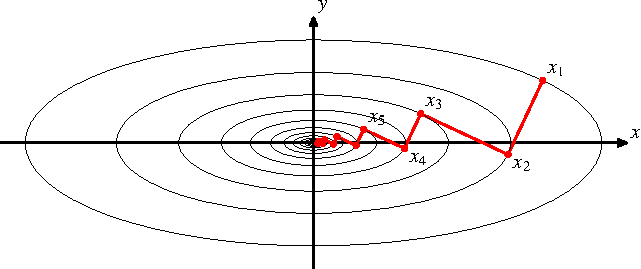
\includegraphics{papers/cg/images/descent-1}
	\caption{Gradient Descent für ellipsenförmige Niveaulinien (schlechte Konditionierung) in 2D. 
		Abbildung aus dem Seminar Buch von 2014 \cite{cg:book:hpc}.}
	\label{cg:abb:steepest_descent}
\end{figure}

\subsection{Minimierungsproblem \label{cg:subsection:Minimierungsproblem}}

Eine Lösung für $x$ kann durch Minimieren von
\begin{equation}
\Phi(x) = \frac{1}{2} x^T A x - x^T b
\end{equation}
gefunden werden.
Der folgende Beweis zeigt, wieso dies ein sinnvoller Ansatz ist.

\begin{proof}[Beweis]
	Wir definieren eine zweite Variable $z = x + \lambda y$, was uns erlaubt die folgende Differenz auszurechnen
	\begin{align}
	\Phi(z) - \Phi(x) 
	&= 
	\frac{1}{2} \left(x + \lambda y\right) ^T A \left(x + \lambda y\right)  - \left(x + \lambda y\right) ^T b
	- 
	\frac{1}{2} x^T A x + x^T b 
	\\
	&= 
	\frac{1}{2} \left(x^T A x + x^T A \lambda y + \lambda y^T A x + \lambda y^T A \lambda y\right) 
	-
	x^T b - \lambda y^T b
	- 
	\frac{1}{2} x^T A x + x^T b .	
	\end{align}
	Da $A$ symmetrisch ist, können die Terme $x^T A \lambda y$ und $\lambda y^T A x$ zusammengefasst werden (analog zur binomischen Formel)
	\begin{align}
	\Phi(z) - \Phi(x) 
	&= 
	\frac{1}{2}\cancel{ x^T A x} + x^T A \lambda y + \frac{1}{2} \lambda y^T A \lambda y
	-
	\bcancel{x^T b} - \lambda y^T b
	- 
	\frac{1}{2}\cancel{ x^T A x} + \bcancel{x^T b} \\
	&=
	\lambda x^T A y	+ \frac{1}{2} {\lambda}^2 y^T A y - \lambda y^T b \\
	&=
	\frac{{\lambda}^2}{2} y^T A y + \lambda y^T \left(Ax -b \right) .
	\end{align}
	Nun können wir den Beweis führen, indem wir $\Phi(z) \ge \Phi(x)$ setzen (da $\Phi(x)$ ja minimiert wird)
	\begin{align}
	\Phi(z) &\ge \Phi(x) 
	\\
	\Phi(z) &= \frac{{\lambda}^2}{2} y^T A y + \lambda y^T \left(Ax -b \right) + \Phi(x) 
	\\
	0 &\le \frac{{\lambda}^2}{2} y^T A y + \lambda y^T \left(Ax - b \right) \quad \forall \quad y \in \mathbb{R}^N  .
	\end{align}
	Der erste Term ist dabei quadratisch in $\lambda$, $A$ ist positiv definit und somit ist immer $\frac{{\lambda}^2}{2} y^T A y \ge 0$.
	Beim zweiten Term ist diese Bedingung nur erfüllt, wenn $Ax - b = 0$ für alle $y$.
	Damit ist bewiesen, dass dann eine Lösung für die Gleichung $Ax = b$ durch Minimierung von $\Phi(x)$ gefunden wird.
\end{proof}

\subsection{Berechnung der Schrittweite \label{cg:subsection:schrittweite}}
Falls eine Suchrichtung gegeben ist, kann die optimale Schrittweite bestimmt werden um $\Phi(x)$ minimal werden zu lassen.
Als Suchrichtung bezeichnen wir die Richtung, in welcher das aktuelle $x$ verbessert werden soll.
Wir suchen also ausgehend vom aktuellen $x$ in dieser Richtung nach einem minimalen $\Phi(x)$.
Gegeben: 
\begin{itemize}
	\item Aktueller Index $k$
	\item Suchrichtung $d_k$
	\item Startpunkt $x_k$
\end{itemize}
Wir suchen nun die optimale Schrittweite $\alpha$, um möglichst nahe an die Lösung zu kommen in der gegebenen Suchrichtung.
Dazu stellen wir wieder ein Minimierungsproblem auf
\begin{align}
	\Phi(x_k + \alpha d_k) 
	&= 
	\frac{1}{2} x_k^T A x_k + \alpha x_k^T A d_k + \frac{1}{2} {\alpha}^2 d_k^T A d_k
	-
	x_k^T b - \alpha d_k^T b \\
	&= \frac{1}{2} {\alpha}^2 d_k^T A d_k + \alpha \left( x_k^T A d_k - d_k^T b \right) + \frac{1}{2} x_k^T A x_k -	x_k^T b.
\end{align}
Durch die Symmetrie von $A$ gilt $x_k^T A d_k = d_k^T A x_k$ und man kann das Minimierungsproblem weiter vereinfachen zu
\begin{equation}
	\Phi(x_k + \alpha d_k) = \frac{1}{2} {\alpha}^2 d_k^T A d_k + \alpha d_k^T\left( A x_k - b \right) + \frac{1}{2} x_k^T \left( A x_k - b \right).
\end{equation}
Hier haben wir eine quadratische Gleichung in $\alpha$, welche einer nach oben geöffneten Parabel entspricht (da $d_k^T A d_k \ge 0$).
Somit ist es möglich ein klares Minimum zu finden, indem wir die Gleichung nach $\alpha$ ableiten und null setzen:
\begin{equation}
	\frac{\partial \Phi(x_k + \alpha d_k) }{\partial \alpha}
	= 
	\alpha  d_k^T A d_k + d_k^T\left( A x_k - b \right)
	=
	0 .
\end{equation}
Dies ergibt für $\alpha$ 
\begin{equation}
	\alpha
	=
	\frac{d_k^T \left(b - A x_k\right)}{d_k^T A d_k}.
\end{equation}
Wenn wir nun den Fehler der momentanen Approximation als Residuum $r_k = b - A x_k$ bezeichnen, erhalten wir
\begin{equation}
	\alpha
	= 
	\frac{\langle d_k , r_k \rangle}{\langle d_k , d_k \rangle_A},
\end{equation}
wobei $\langle d_k , d_k \rangle_A = d_k^T A d_k$ das verallgemeinerte Skalarprodukt zu $A$ darstellt.
Somit haben wir nun die optimale Schrittlänge gefunden.

Daraus lässt sich nun der nächste Punkt $x_{k+1}$ berechnen als
\begin{equation}
	x_{k+1} = x_k + \frac{\langle d_k , r_k \rangle}{\langle d_k , d_k \rangle_A} d_k.
\end{equation}

\subsection{Berechnung des Gradienten}
Die neue Suchrichtung $d_{k+1}$ entspricht dem negativen Gradienten von $\Phi(x_{k+1})$.
Dieser Gradient lässt sich berechnen als
\begin{equation}
	d_{k+1} = - \nabla \Phi(x_{k+1}) = - \nabla \left( \frac{1}{2} x_{k+1}^T A x_{k+1} - x_{k+1}^T b \right) = -(Ax_{k+1} - b) = b - Ax_{k+1},
\end{equation}
Wobei zur Berechnung der quadratischen Ableitung Lemma \ref{buch:qm:lemma:gradsquare} zur Anwendung kommt.
\begin{beobachtung} \label{cg:beob:residuum}
	Somit ist die neue Abstiegsrichtung identisch zum neuen Residuum $r_{k+1}$.
\end{beobachtung}

\subsection{Probleme beim Gradient Descent}
Mit den hier hergeleiteten Resultaten kann eine approximative Lösung gefunden werden.
Die Konvergenzgeschwindigkeit ist allerdings stark abhängig von $A$.
Das Beispiel in Abbildung \ref{cg:abb:steepest_descent} zeigt (in 2D), wie Gradient Descent bei ovalen Niveaulinien zu oszillieren beginnt.
Die Konvergenz ist also in diesem Fall sehr langsam, die exakte Lösung wird nie erreicht.
Falls die Niveaulinien allerdings eher rund sind, erhöht sich die Konvergenzgeschwindigkeit.

Diese Probleme werden mit der Erweiterung zum CG-Algorithmus behoben.

\subsection{Beispiel zur Motivation der $A$-Orthogonalität} \label{cg:subsec:aortho}
Das folgende Beispiel soll ausgehend von Gradient Descent die Motivation liefern, weshalb im CG-Algorithmus die $A$-Orthogonalität wichtig ist.
Unter $A$-Orthogonalität ($\perp_A$) zweier Vektoren versteht man, dass deren verallgemeinertes Skalarprodukt zu $A$ verschwindet:
\begin{equation}
	a \perp_A b \Longrightarrow a^T A b = \langle a , b \rangle_A = 0.
\end{equation}
Richtungen welche $A$-orthogonal stehen, werden auch konjugiert bezüglich $A$ genannt.
Dies erklärt den Namen des CG-Verfahrens.
Für das Beispiel definieren wir $A$, $b$, $x_1$ und berechnen $x_2$:
\begin{align}\nonumber
	A 	&= 		\begin{pmatrix}
				4 & 0\\
				0 & 9 
				\end{pmatrix} \nonumber\\
	b 	&= 		\begin{pmatrix}
				0\\
				0
				\end{pmatrix} \nonumber\\
	x_1 &= 		\begin{pmatrix}
				1\\
				1
				\end{pmatrix} \nonumber\\
	r_1	&= 		b - A x_1 = - 	\begin{pmatrix}
								4\\
								9
								\end{pmatrix} \nonumber\\
	d_1 &= r_1 \nonumber\\
	x_2 &= x_1 + \frac{\langle r_1 , r_1 \rangle}{\langle r_1 , r_1 \rangle_A} r_1 = 	\begin{pmatrix}
																						0.51\\
																						-0.1
																						\end{pmatrix}. \\
\end{align}
Dieses Gleichungssystem hat den Nullpunkt als Lösung $x = \begin{pmatrix}0\\0\end{pmatrix}$.
Um im nächsten Schritt eine Lösung finden zu können, müsste die nächste Abstiegsrichtung dem Vektor von $x_2$ zum Ursprung entsprechen.
Wenn wir das $A$-Skalarprodukt von $-x_2$ und $d_1$ berechnen, verschwindet dieses:
\begin{equation}
	\langle -x_2 , d_1 \rangle_A = 	-x_2^T A d_1 = 
		\begin{pmatrix} 0.51 & -0.1 \end{pmatrix} 
		\begin{pmatrix} 4 & 0\\
						0 & 9 
		\end{pmatrix} 
		\begin{pmatrix} -4\\
						-9 
		\end{pmatrix} = 0 \nonumber
\end{equation}
was der $A$-Orthogonalität entspricht.
Damit ist gezeigt, dass die optimale zweite Abstiegsrichtung $A$-orthogonal zur ersten Abstiegsrichtung wäre.
Somit ist die $A$-Orthogonalität das entscheidende Konzept um dem CG-Algorithmus zu ermöglichen in $N$-Schritten eine exakte Lösung zu finden.
Abbildung \ref{cg:abb:cg1} zeigt das Resultat einer solchen optimalen Wahl der zweiten Abstiegsrichtung.
\section{Herleitung des Algorithmus}
\label{cg:section:herleitung}
\rhead{Herleitung des Algorithmus}

\subsection{Intuition}
%TODO grafics "Abstieg auf Koordinatenachsen"

\subsection{Optimale Suchrichtung \label{cg:subsection:suchrichtung}}

Nun muss nur noch die optimale nächste Suchrichtung $d_{k+1}$ gefunden werden.
Damit jeder Schritt das Problem um eine Dimension reduziert, muss jede neue Suchrichtung orthogonal im Sinne von $A$ auf allen bisherigen Richtungen stehen. %TODO Grafik
Dies ist erreicht wenn das Residuum $r_k$ mithilfe des Gram-Schmidt-Orthogonalisierungsverfahren auf $d_k$ orthogonalisiert wird %TODO beweis dafür  (S. 80)
\begin{equation}
d_{k+1}
= 
r_{k+1} - \frac{\langle d_k , r_{k+1} \rangle_A}{\langle d_k , d_k \rangle_A} d_k.
\end{equation}

\subsection{Genügt Orthogonalisierung auf der letzten Richtung?}


\section{Ergebnisse}
\label{cg:section:ergebnisse}
\rhead{Ergebnisse}

In diesem Abschnitt werden kurz die Ergebnisse der Implementation erwähnt.
Die Implementation wurde mit Python erstellt und ermöglicht eine Konvergenzuntersuchung.
Es zeigte sich, dass die Konvergenzgeschwindigkeit stark von der Konditionierung von $A$ abhängt.
Die Konditionierung wird mit der Konditionszahl $\kappa_A$ gemessen, welche das Verhältnis vom grössten zum kleinsten Eigenwert von $A$ bezeichnet.
Je grösser $\kappa_A$ ist, desto schwerer ist ein Problem zu lösen.
Optimal wäre ein $\kappa_A = 1$, wobei dann die Niveaulininen die Form einer Hyperkugel (Kreis in 2D) annehmen.

Alle nachfolgenden Beispiele lösen ein $N=1000$-dimensionales Problem, was in einer $1000 \times 1000$ Matrix $A$ resultiert.
In Abbildung \ref{cg:abb:slow_conv} sieht man ein Beispiel einer schlechten Konditionierung.
Dabei wird bei etwa $k=200$ Schritten eine Genauigkeit von $10^{-3}$ erreicht.
Abbildung \ref{cg:abb:fast_conv} dagegen zeigt das Verhalten bei sehr guter Konditionierung.
Hier wird bereits nach wenigen Schritten die Genauigkeit von $10^{-3}$ erreicht.
Also haben wir einen starken Einfluss der Konditionierung auf die Konvergenzgeschwindigkeit.
Falls schnelle Konvergenz verlangt wird, kann sich somit eine Präkonditionierung lohnen, welche $\kappa_A$ verbessern würde.

Zum Abschluss zeigt Abbildung \ref{cg:abb:no_conv} was passiert wenn $A$ nicht positiv definit ist.
Das aufgestellte Minimierungsproblem von \ref{cg:subsection:Minimierungsproblem} stimmt dadurch nicht und der CG-Algorithmus scheitert.
Dies äussert sich durch starke Oszillazion bei hohem absolutem Fehler.

\begin{figure}	
	\centering
	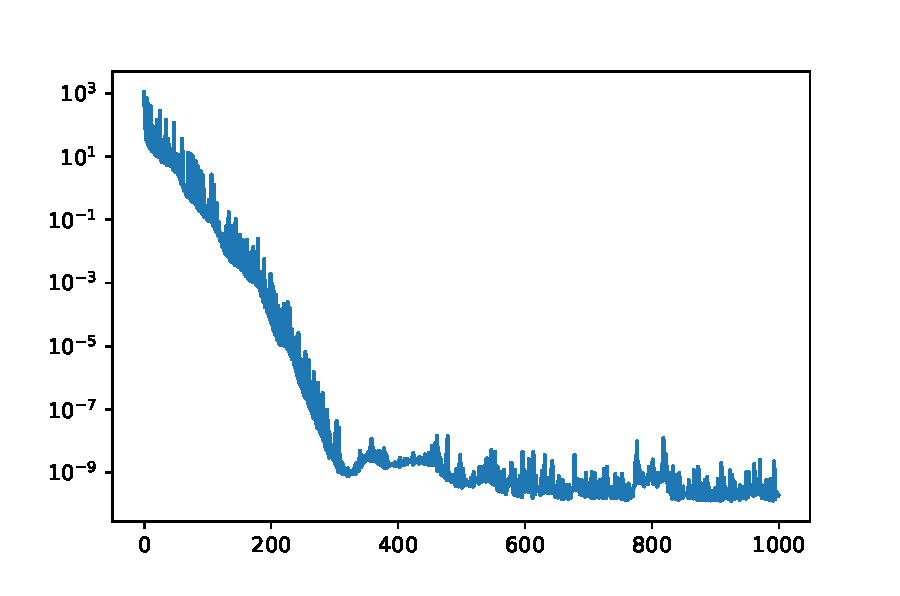
\includegraphics[width=0.8\textwidth]{papers/cg/images/convergence_k_750000}
	\caption{Betrachtung des absoluten Fehlers in Abhängigkeit der Anzahl Schritte bei schlechte Konditionierung ($\kappa_A=750000$).}
	\label{cg:abb:slow_conv}
\end{figure}

\begin{figure}	
	\centering
	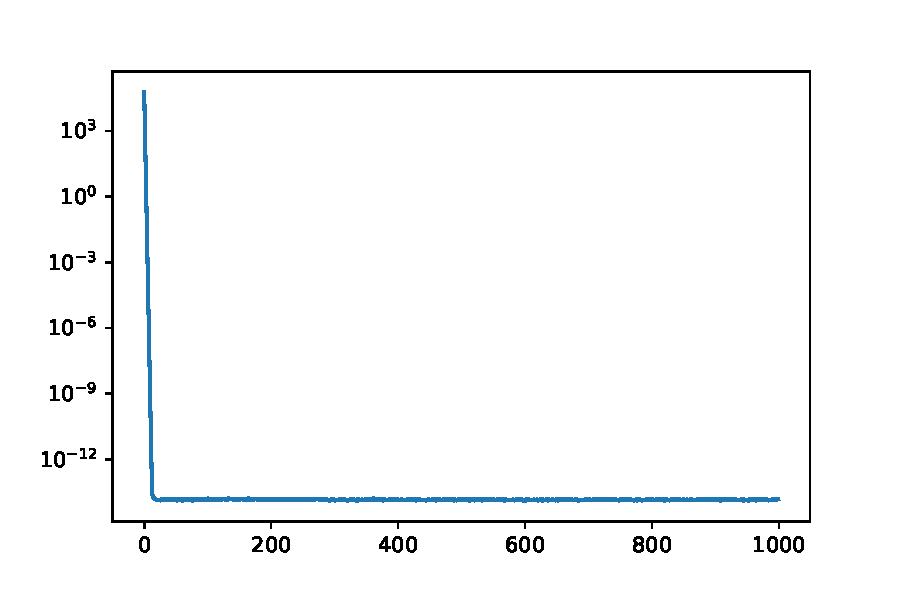
\includegraphics[width=0.8\textwidth]{papers/cg/images/convergence_k_1_1}
	\caption{Betrachtung des absoluten Fehlers in Abhängigkeit der Anzahl Schritte bei guter Konditionierung ($\kappa_A=1.1$).}
	\label{cg:abb:fast_conv}
\end{figure}

\begin{figure}	
	\centering
	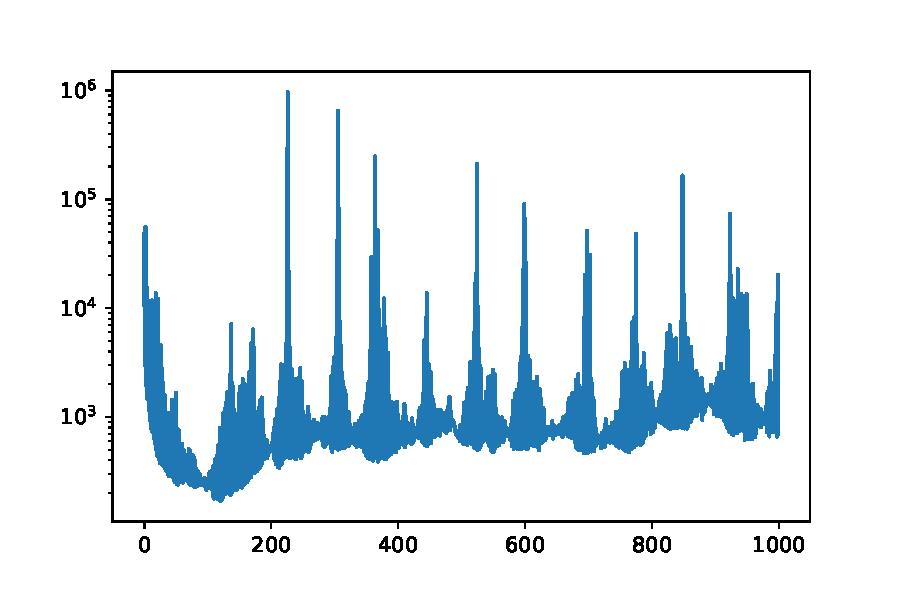
\includegraphics[width=0.8\textwidth]{papers/cg/images/no_convergence}
	\caption{Betrachtung des absoluten Fehlers in Abhängigkeit der Anzahl Schritte falls $A$ nicht positiv definit ist. 
			Es ergibt sich keine Konvergenz.}
	\label{cg:abb:no_conv}
\end{figure}

\subsection{Fazit}
Die hier vorgestellte Methode der konjugierten Gradienten (CG) liefert schnelle, genaue Resultate für grosse lineare Gleichungssysteme.
Besonders interessant ist, dass theoretisch sogar die exakte Lösung gefunden wird (nach $N$ Schritten).
In der Implementation stellt sich dies aufgrund der begrenzten digitalen Genauigkeit natürlich als unmöglich heraus.
Trotzdem ist diese Eigenschaft hilfreich, da es eine fixe Obergrenze für die Anzahl Schritte darstellt.
Falls die Kondition gut ist (was häufig der Fall ist), ist die Konvergenz sehr schnell und es werden deutlich weniger als $N$ Schritte benötigt.

\printbibliography[heading=subbibliography]
\end{refsection}
